% \section{Evaluation}
\label{sec:eval}

The evaluation of the final \emph{Canary-1B-v2} model is conducted using the benchmark suites introduced in Section~\ref{sec:evaluation-benchmarks}. For comparative analysis, we consider several strong baselines: \emph{Whisper-large-v3} (1.55B), \emph{seamless-m4t-v2-large} (2.3B), and \emph{seamless-m4t-medium} (1.2B), as they are the closest in scale to \emph{Canary-1B-v2} among seamless speech models. In addition, we include \emph{Voxtral-Mini-3B-2507}\cite{liu2025voxtral} (3B) and \emph{Phi-4-multimodal-instruct}\cite{abouelenin2025phi4multimodal} (5.6B), two multimodal and LLM-based systems, in order to highlight the trade-offs between accuracy and inference efficiency where \emph{Canary-1B-v2} provides an advantage. Our second release, \emph{Parakeet-TDT-0.6B-v3}, is likewise included in the multilingual ASR evaluations.



Multilingual evaluations in this section are reported under two complementary settings:  
\begin{enumerate}
    \item \textbf{All supported languages:} 24 total, excluding Latvian, which is not supported by \emph{seamless-m4t-v2-large} or \emph{seamless-m4t-medium}.  
    \item \textbf{Common languages:} 6 shared by all compared models (\emph{en}, \emph{fr}, \emph{de}, \emph{it}, \emph{pt}, and \emph{es}).  
\end{enumerate}


\subsection{ASR Performance}

For ASR performance evaluation, we report normalized WER (\%). We use the Hugging Face Open Automatic Speech Recognition Leaderboard normalizers\footnote{\url{https://github.com/huggingface/open_asr_leaderboard/tree/main/normalizer}}: the English normalizer for English test sets, and the newly added multilingual normalizer for non-English test sets. Both remove punctuation and lowercase the text. The English normalizer further performs richer, language-specific normalization (e.g., numbers, abbreviations, currencies), whereas the multilingual normalizer emphasizes cross-language consistency by replacing symbols and punctuation-like markers with spaces and by mapping or stripping diacritics to their base forms.


\subsubsection{English ASR (HuggingFace Leaderboard) Performance}

Table~\ref{tab:asr-performance} presents the results for the Hugging Face Leaderboard datasets, calculated with the official repository and reported on the Hugging Face Open ASR Leaderboard. Notably, \emph{Canary-1B-v2} outperforms \emph{Whisper-large-v3} on the official average WER metric, while also achieving remarkable inference efficiency. With an RTFx of 749, \emph{Canary-1B-v2} runs approximately 7--10 times faster than the other evaluated models, highlighting its strength in balancing accuracy with throughput efficiency.

Additionally, \emph{Parakeet-TDT-0.6B-v3} attains the highest throughput among all systems (RTFx \(=3332.74\)) while maintaining a low average WER of \(6.32\%\), within \(0.18\) absolute points of \emph{Phi-4-multimodal-instruct} (\(6.14\%\)). This corresponds to \(\approx 54\times\) faster inference than \emph{Phi-4-multimodal-instruct}, combining near–state-of-the-art accuracy with extreme throughput.

\begin{table}[ht]
\centering
\resizebox{\textwidth}{!}{%
\begin{tabular}{lcccccccccc}
\toprule
\textbf{Model} & \textbf{RTFx} & \textbf{Avg WER} & \textbf{AMI} & \textbf{Earnings22} & \textbf{Gigaspeech} & \textbf{LS Clean} & \textbf{LS Other} & \textbf{SPGI} & \textbf{TED-LIUM} & \textbf{VoxPopuli} \\
\midrule
\emph{Whisper-large-v3}          & 145.51 & 7.44 & 15.95 & 11.29 & 10.02 & 2.01 & 3.91 & 2.94 & 3.86 & 9.54 \\
\emph{Voxtral-Mini-3B-2507}      & 109.86 & 7.05 & 16.31 & 10.65 & 10.24 & 1.89 & 4.08 & 2.37 & 3.70 & 7.14 \\
\emph{Phi-4-multimodal-instruct} &  62.12 & 6.14 & 11.45 & 10.50 &  9.77 & 1.67 & 3.82 & 3.11 & 2.89 & 5.93 \\
\midrule
\emph{Parakeet-TDT-0.6B-v3}              & 3332.74 & 6.32 & 11.39 & 11.19 & 9.57 & 1.92 & 3.59 & 3.98 & 2.8 & 6.09 \\
\midrule
\emph{Canary-1B-v2}              & 749.00 & 7.15 & 16.01 & 11.79 & 10.82 & 2.18 & 3.56 & 2.28 & 4.29 & 6.25 \\
\bottomrule
\end{tabular}%
}
\vspace{10pt}
\caption{ASR performance (WER \%) and inference efficiency (RTFx) on Hugging Face OpenASR Leaderboard benchmarks.}
\label{tab:asr-performance}
\end{table}


\subsubsection{Multilingual ASR Performance}

As is seen in Figure~\ref{fig:multilingual-asr}, \emph{Canary-1B-v2} demonstrates consistently strong multilingual ASR performance across both the full 24-language set and the common 6-language subset. On the full evaluation, computed as an average across three different datasets (FLEURS, CoVoST, MLS), it achieves an average WER of around 8.1\%, outperforming \emph{whisper-large-v3} (9.9\%) and \emph{seamless-m4t-medium} (12.0\%), while remaining only slightly behind the much larger and heavier \emph{seamless-m4t-v2-large} (7.2\%). On the common-language evaluation, also averaged across the same three datasets, \emph{Canary-1B-v2} reaches 5.2\% WER compared to 5.8\% for \emph{whisper-large-v3} and 8.2\% for \emph{seamless-m4t-medium}, and in fact slightly outperforms \emph{seamless-m4t-v2-large} (5.3\%). Even though other models are specialized in this smaller set, \emph{Canary-1B-v2} supports 19 additional languages while still matching or surpassing much heavier and LLM-powered baselines.

Additionally, the companion 0.6B model \emph{Parakeet-TDT-0.6B-v3} averages 9.7\% WER across the 24-language evaluation (11.52/9.78/7.83 on FLEURS/CoVoST/MLS), edging past \emph{whisper-large-v3} (9.9\%) while trailing \emph{Canary-1B-v2} (8.1\%) and \emph{seamless-m4t-v2-large} (7.2\%). On the common-language subset it reaches 5.3\% WER (4.37/4.79/6.74), essentially matching \emph{seamless-m4t-v2-large} (5.3\%) and outperforming \emph{whisper-large-v3} (5.8\%).



\begin{figure}[htbp]
    \centering
    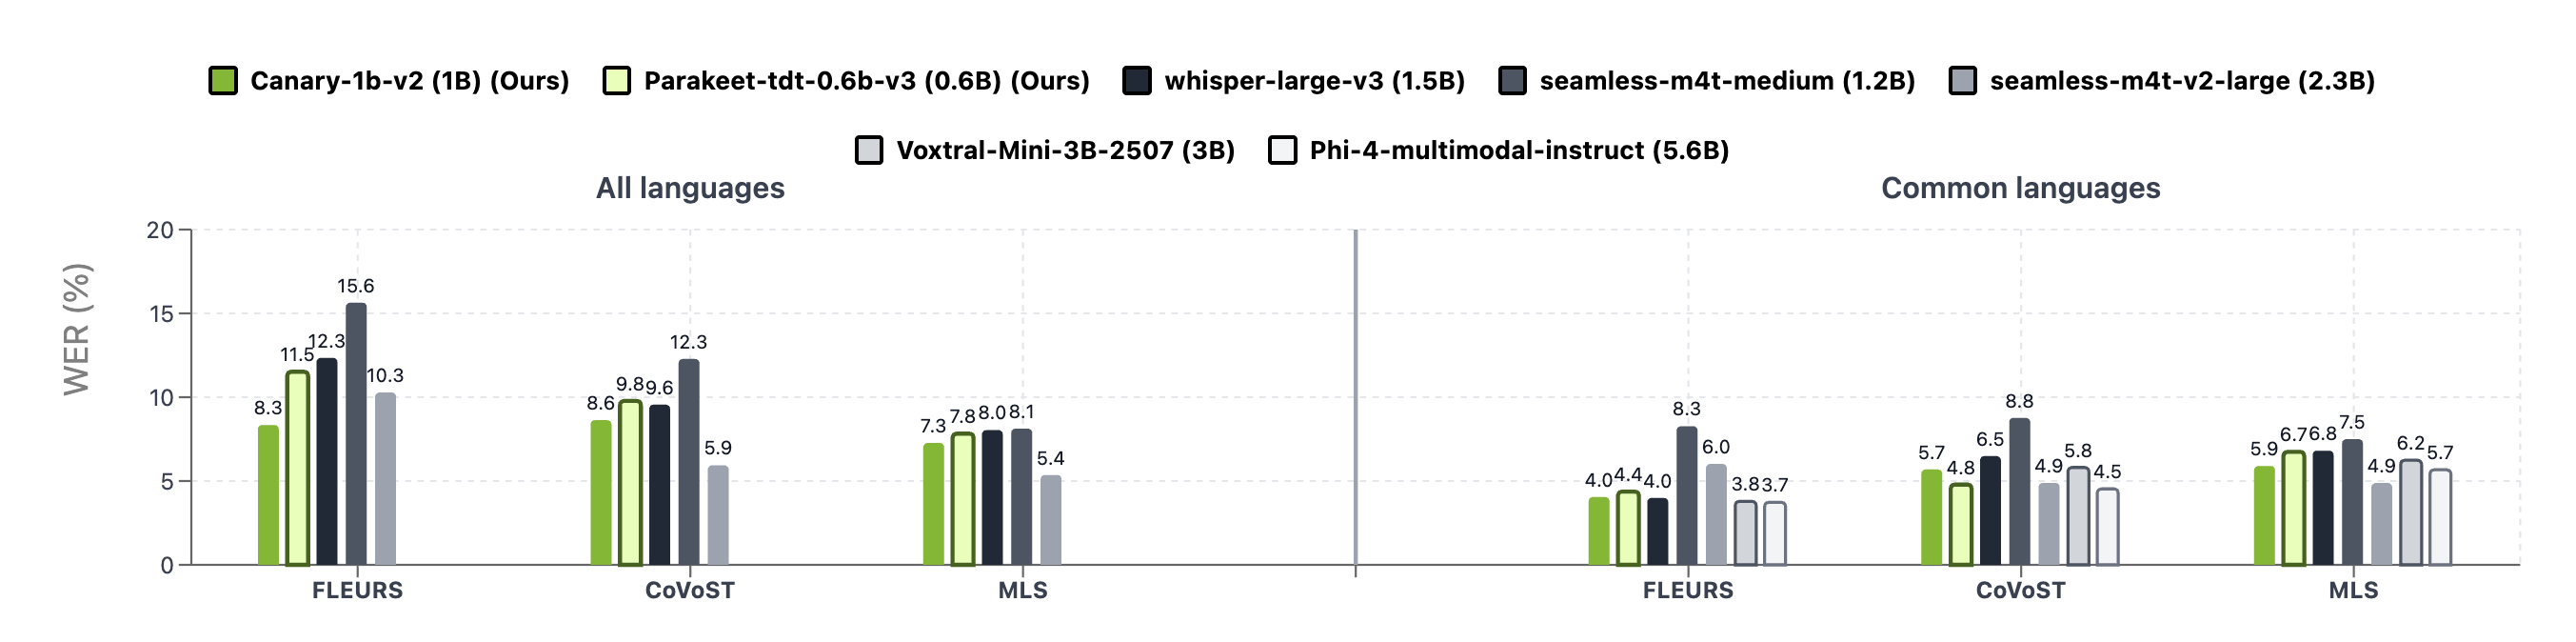
\includegraphics[width=0.99\linewidth]{images/eval_asr.png}
    \caption{Multilingual ASR performance of \emph{Canary-1B-v2} and \emph{Parakeet-TDT-0.6B-v3} compared to baseline models on both 24-language and 6-language subsets.}
    \label{fig:multilingual-asr}
\end{figure}

Per-language WERs for each evaluation benchmark are provided in the Appendix~\ref{app:eval_details_asr}


\subsubsection{Noise-robustness evaluation}

Table~\ref{tab:noise-robustness} reports the robustness of \emph{Canary-1B-v2} and \emph{Parakeet-TDT-0.6B-v3} across different Signal-to-Noise Ratios (SNR) on the LibriSpeech Clean test set\cite{librispeech}, where MUSAN music and noise samples~\cite{snyder2015musanmusicspeechnoise} were added.

Interestingly, we observe that performance of \emph{Canary-1B-v2} slightly improves when decreasing the SNR from 100 to 25, with WER dropping from 2.18\% to 2.01\%. This suggests that \emph{Canary-1B-v2} benefits from a small amount of background noise, likely due to training on large-scale datasets that naturally include noisy conditions, such as the YouTube subset of the Granary corpus and VoxPopuli, where background noise from live interpreters and other sources is present. This indicates that the model has learned to leverage noisy input scenarios, resulting in improved robustness.  

Complementing this, \emph{Parakeet-TDT-0.6B-v3} is consistently more robust across SNRs (1.92–1.96\% WER from 100 to 25 dB) and outperforming under severe noise with 12.21\% at \(-5\) dB vs 19.38\% for \emph{Canary-1B-v2} (\(\sim\)37\% relative).


\begin{table}[ht]
\centering
\begin{tabular}{lccccccc}
\toprule
\ & \multicolumn{7}{c}{\textbf{SNR (dB)}} \\
\cmidrule(lr){2-8}
\textbf{Model} & \textbf{100} & \textbf{50} & \textbf{25} & \textbf{10} & \textbf{5} & \textbf{0} & \textbf{-5} \\
\midrule
\emph{Parakeet-TDT-0.6B-v3} & \textbf{1.92} & \textbf{1.92} & 1.96 & 2.15 & 2.62 & 4.82 & 12.21 \\
\midrule
\emph{Canary-1B-v2} & 2.18 & 2.16 & \textbf{2.01} & 2.29 & 2.80 & 5.08 & 19.38 \\
\bottomrule
\end{tabular}

\vspace{10pt}

\caption{WER (\%) across different SNR levels on the LibriSpeech Clean test set with MUSAN music and noise samples.}
\label{tab:noise-robustness}
\end{table}






\subsection{AST Performance}

For AST performance we consider two evaluation directions: X$\to$En En and En $\rightarrow X$. We again used the evaluation benchmarks introduced in Section~\ref{sec:evaluation-benchmarks}.

In terms of performance metrics, we report both COMET and BLEU\cite{papineni2002bleu} scores. COMET is used as the primary metric throughout this section, while BLEU scores are reported in Appendix~\ref{app:eval_details_ast_x-en} and \ref{app:eval_details_ast_en-x}. BLEU, being based on $n$-gram overlap, often underestimates semantic adequacy when translations diverge lexically or syntactically from reference sentences but remain valid. This makes BLEU less reliable, especially in multilingual and low-resource settings. COMET, in contrast, leverages pretrained multilingual encoders and human-annotated data, enabling it to better capture semantic similarity and translation quality beyond surface-level word overlap. As such, COMET provides a more faithful reflection of translation performance, while BLEU is included for completeness and comparability with prior work.

\subsubsection{\texorpdfstring{X$\to$En Performance}{X→En Performance}}

As shown in Figure~\ref{fig:ast-x-en}, \emph{Canary-1B-v2} outperforms \emph{whisper-large-v3} and \emph{seamless-m4t-medium} by a large margin across both evaluation benchmarks. On the full-language setting, it achieves 79.28 COMET on FLEURS and 78.14 on CoVoST2, compared to 76.51 / 74.61 for \emph{whisper-large-v3} and 77.30 / 75.64 for \emph{seamless-m4t-medium}. Even against the much larger \emph{seamless-m4t-v2-large} (81.71 / 80.26), \emph{Canary-1B-v2} remains close despite having less than half the parameters.  

On the common-language evaluation, \emph{Canary-1B-v2} continues to perform strongly, reaching 82.41 COMET on FLEURS and 79.07 on CoVoST. This is competitive with the heavier \emph{seamless-m4t-v2-large} (82.84 / 80.16) and even the LLM-powered \emph{Voxtral-Mini-3B-2507} (84.53 / 78.90) and \emph{Phi-4-multimodal-instruct} (84.06 / 80.11). Notably, on the more spontaneous and noisy CoVoST2 dataset, \emph{Canary-1B-v2} performs particularly well (79.07 vs.\ 76.86 for \emph{whisper-large-v3}), increasing the gap over the \emph{whisper} model, comparable to the \emph{Phi-4-multimodal-instruct} (80.11), and even outperforming the \emph{Voxtral-Mini-3B-2507} (78.90). This reflects the robustness learned from large-scale noisy training sources.    


\begin{figure}[htbp]
    \centering
    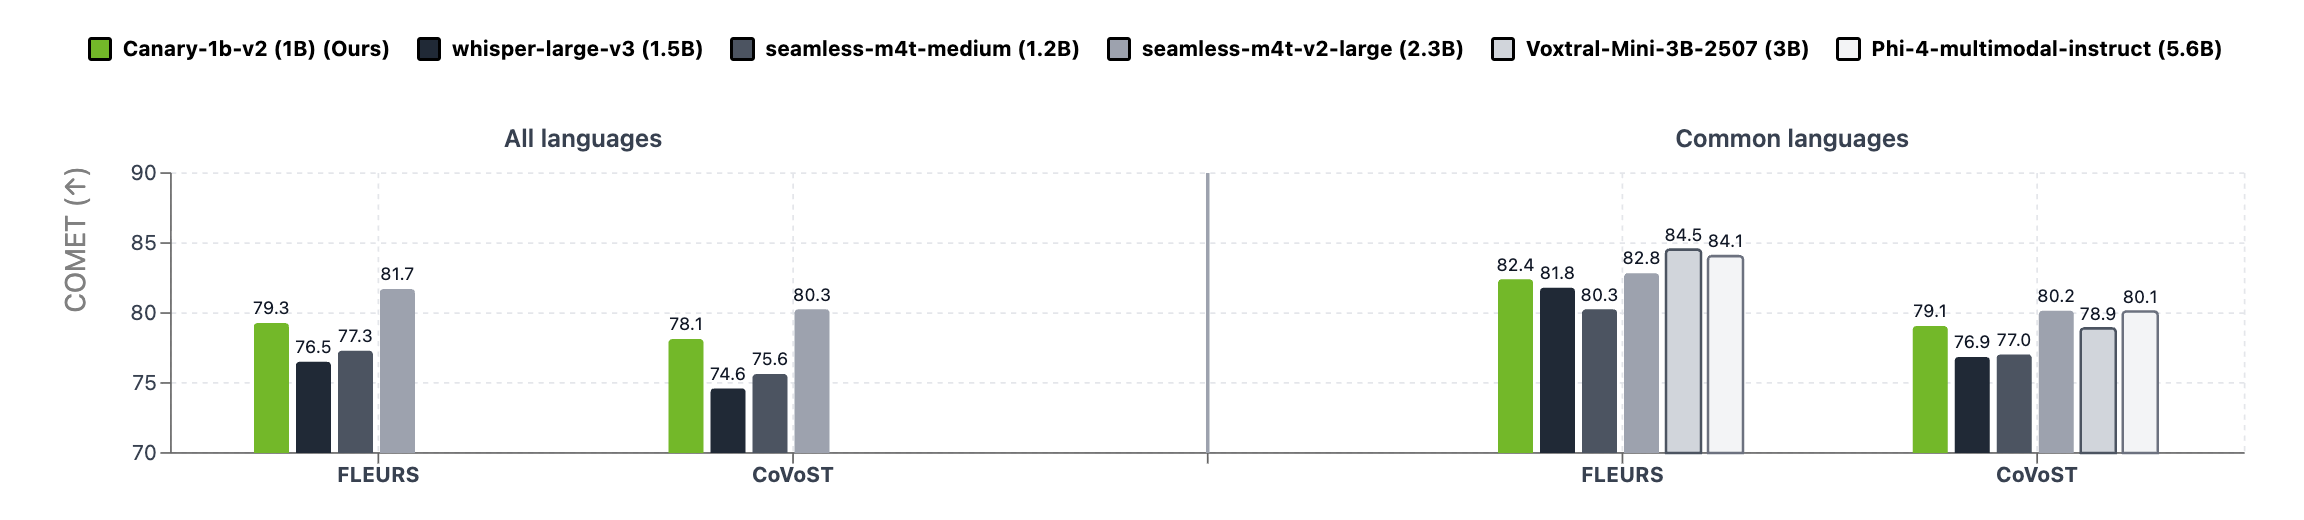
\includegraphics[width=0.99\linewidth]{images/eval_x_en.png}
    \caption{AST (X$\to$En) performance of \emph{Canary-1B-v2} compared to baseline models on both 24-language and 6-language subsets.}
    \label{fig:ast-x-en}
\end{figure}

\subsubsection{\texorpdfstring{En$\to$X Performance}{En→X Performance}}

As shown in Figure~\ref{fig:ast-en-x}, \emph{Canary-1B-v2} achieves strong En$\to$X performance. On FLEURS, it remains on par with the much larger \emph{seamless-m4t-v2-large} in the all-language setting (84.47 vs.\ 84.85 COMET) and even slightly outperforms all compared models in the supported-language evaluation (83.79 vs.\ 83.56 for \emph{seamless-m4t-v2-large}, 82.20 for \emph{Phi-4}, and 83.56 for \emph{Voxtral-Mini-3B-2507}). On CoVoST2, however, \emph{Canary-1B-v2} lags behind \emph{seamless-m4t-v2-large} (80.03 vs.\ 82.66 in the all-language setting, and 78.37 vs.\ 81.30 in the supported-language evaluation). A possible explanation is that while the En$\to$X training data covers diverse domains, the X-language ASR pathways were more strongly shaped by narrower-domain data, leading the decoder to generalize less effectively to spontaneous CoVoST speech.


\begin{figure}[htbp]
    \centering
    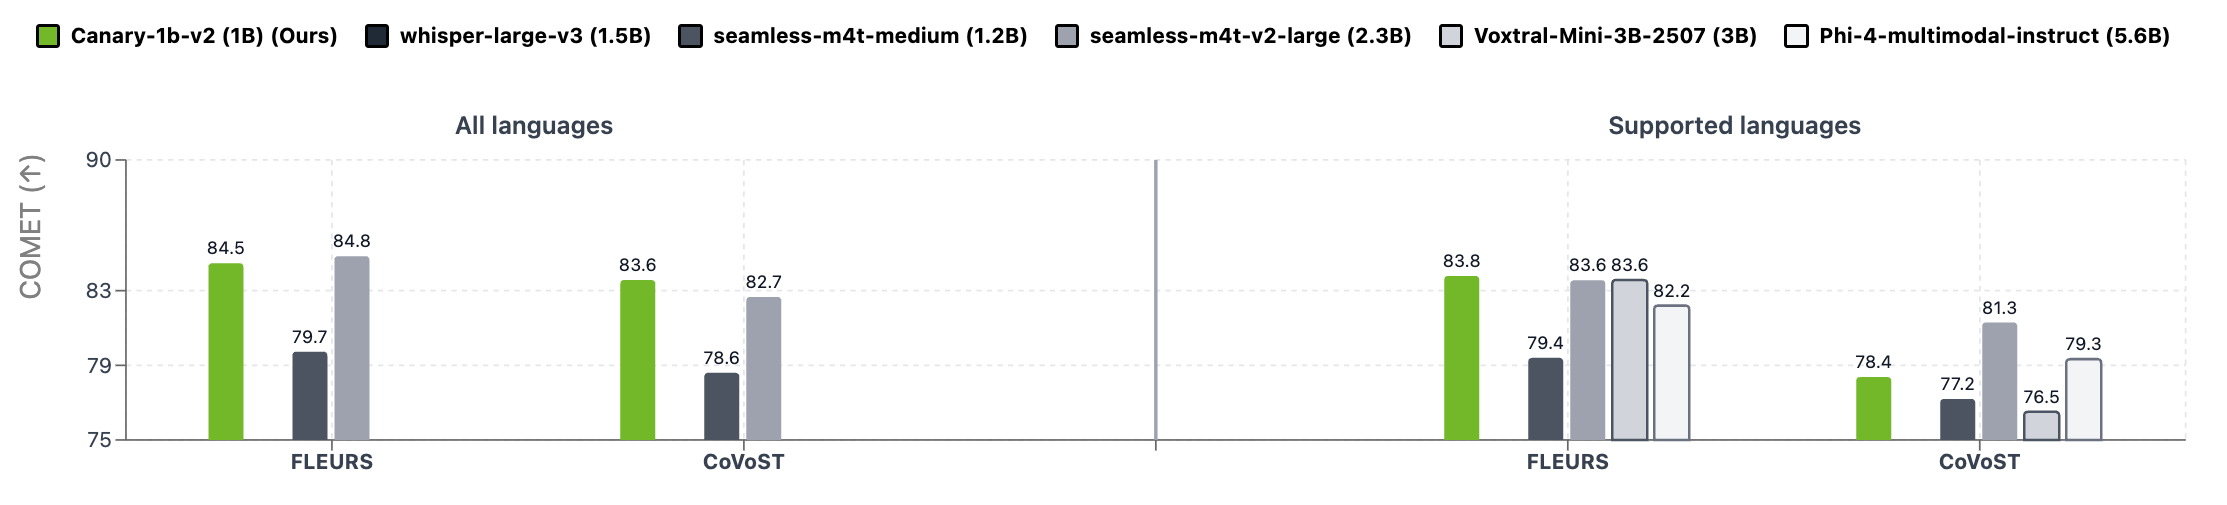
\includegraphics[width=0.99\linewidth]{images/eval_en_x.png}
    \caption{AST (En$\to$X) performance of \emph{Canary-1B-v2} compared to baseline models on both 24-language and 6-language subsets.}
    \label{fig:ast-en-x}
\end{figure}

\subsection{nGPT and FastConformer comparison}
To better understand the capabilities of nGPT as an encoder, we trained models of different scales on the Granary datasets. These experiments were designed to assess how well nGPT scales and how it compares to the FastConformer baseline across ASR and AST benchmarks.

As shown in Table \ref{tab:asr-ast-fc-ngpt}, scaling from 1B to 3B parameters consistently improved performance. The 3B-parameter nGPT model demonstrated stronger generalization across tasks, with especially notable gains on the challenging X→EN translation benchmark—where FastConformer struggled most. Importantly, the 3B model achieved these results within a single training stage and only 100k steps. While the 1B model falls short of the 3B across tasks, it still shows the same generalization trend and remains competitive, particularly on translation.

In contrast, FastConformer required a more elaborate multi-stage training regime to achieve strong results. With sufficient fine-tuning, however, it was able to surpass nGPT in all tasks. This highlights a key distinction: nGPT is a data-hungry model that thrives under large-scale training and quickly reaches competitive performance, whereas FastConformer benefits more from fine-tuning and exhibits greater relative improvements in low-data scenarios.


\begin{table}[t]
\centering
\small
\begin{threeparttable}

% (a) ASR
\begin{subtable}{\textwidth}
\centering
\begin{tabularx}{\textwidth}{l l YYYY}
\toprule
\textbf{Model} & \textbf{Regime} &
HF Leaderboard (En) & FLEURS (25) & MLS (5) & CoVoST2 (13) \\
\midrule
FC 1B   & 1st stage        & 7.73\% & 10.66\% & 7.35\% & 8.11\% \\
nGPT 1B & 1st stage        & 8.94\% &  9.94\% & 8.11\% &  9.96\% \\
nGPT 3B & 1st stage        & 7.73\% & 10.18\% & 8.35\% & 10.48\% \\
\midrule

FC 1B   & 3-stage (15k HQ) & 7.15\% & 8.69\% & 7.11\% & 10.33\% \\
nGPT 3B & 2-stage (15k HQ) & 7.32\% & 10.31\% & 8.32\% & 10.30\% \\
\bottomrule
\end{tabularx}
\caption{ASR results (WER). Lower is better.}
\end{subtable}

\vspace{10pt}

% (b) AST X->En
\begin{subtable}{\textwidth}
\centering
\begin{tabularx}{\textwidth}{l l YY}
\toprule
\textbf{Model} & \textbf{Regime} &
FLEURS (24) & CoVoST2 (11) \\
\midrule
FC   1B   & 1st stage        & 73.18 & 75.39 \\
nGPT 1B & 1st stage        & 76.72 & 74.02 \\
nGPT 3B & 1st stage        & 78.36 & 75.75 \\
\midrule
FC   1B   & 3-stage (15k HQ) & 79.27 & 76.82 \\
nGPT 3B & 2-stage (15k HQ) & 79.14 & 75.90 \\
\bottomrule
\end{tabularx}
\caption{AST (X$\to$En) results (COMET). Higher is better.}
\end{subtable}

\vspace{10pt}

% (c) AST En->X
\begin{subtable}{\textwidth}
\centering
\begin{tabularx}{\textwidth}{l l YY}
\toprule
\textbf{Model} & \textbf{Regime} &
FLEURS (24) & CoVoST2 (5) \\
\midrule
FC 1B   & 1st stage        & 84.30 & 80.63 \\
nGPT 1B & 1st stage        & 83.05 & 78.31 \\
nGPT 3B & 1st stage        & 84.22 & 80.00 \\
\midrule
FC 1B   & 3-stage (15k HQ) & 84.38 & 80.32 \\
nGPT 3B & 2-stage (15k HQ) & 84.28 & 79.48 \\
\bottomrule
\end{tabularx}
\caption{AST (En$\to$X) results (COMET). Higher is better.}
\end{subtable}

\caption{Comparison of FC and nGPT across training regimes on ASR and AST benchmarks.}
\label{tab:asr-ast-fc-ngpt}
\begin{tablenotes}
\centering
\small
\item[$^{*}$] COMET scores computed with \texttt{Unbabel/wmt22-comet-da}.
\end{tablenotes}

\end{threeparttable}
\end{table}


\subsection{Longform inference}
Neural encoders are typically trained on relatively short input sequences, which means they often fail to generalize well when faced with significantly longer contexts at inference time. For ASR, this limitation becomes especially clear when transcribing utterances beyond the average training length (e.g., >40 seconds). As context length grows, models exhibit degraded stability and accuracy, making it essential to explore strategies that overcome this bottleneck.

One class of solutions modifies the inference procedure rather than the model architecture itself. A common approach is local attention \cite{rekesh2023fast}, where each query token attends only to a fixed-size window of neighboring tokens instead of the entire sequence. This sliding-window design reduces quadratic attention costs and stabilizes inference on long inputs, while still capturing the local dependencies most critical for recognition tasks. In practice, such methods can be readily applied in models with CTC or RNN-T heads, making them an effective strategy for scaling ASR systems to longer contexts. The other method is chunking mechanism in which audio is divided into smaller segments that are transcribed separately and then merged and it can easily be adapted to encoder–decoder architectures.

\subsubsection{Chunk based approach}

For our current FastConformer encoder paired with a Transformer decoder, we employed a dynamic parallel chunking mechanism to enable efficient long-form inference. Each input audio file is segmented into chunks of 30–40 seconds, where the exact length is chosen dynamically to minimize padding in the final chunk. To preserve continuity across boundaries, adjacent chunks overlap by 1 second.

The chunked segments are then fed into the model in parallel as separate entries within a batch. After the model produces transcriptions for all segments, the outputs are merged into a single hypothesis. To resolve overlapping regions, we apply a Longest Common Subsequence (LCS) algorithm at the token level, ensuring that duplicated text in the overlap regions is removed from the final transcript.

For very long recordings (longer than one hour), we further segment the audio into hour-long blocks, each processed independently using the same chunking and merging procedure. This hierarchical design ensures scalability to arbitrarily long audio while maintaining both efficiency and transcription quality.
% put this in the preamble

   % for spanning rows/cols
We compared this method with chunking inference without overlap, where fixed audio chunks were processed sequentially through the model one by one, and observed clear performance gains. Table~\ref{tab:chunking_results} summarizes the results. Parallel chunking achieves lower WER and significantly higher RTFx on both benchmarks compared to script-based sequential chunking. On the Earnings22 dataset, WER improved from 15.61\% to 13.93\%, while RTFx increased almost 4×. Similarly, on the TAL(10h) dataset, WER dropped from 16.62\% to 10.12\%, and RTFx more than doubled.

\begin{table}[ht]
\centering
\caption{Comparison of two chunking mechanisms for long-form inference. In parallel chunking(ours), audio is split into overlapping chunks that are processed simultaneously within a batch, with overlaps later merged to maintain continuity. In \textit{sequential chunking}, fixed-length chunks are processed one by one without overlap, and outputs are concatenated directly.}
\begin{tabular}{|l|c c|c c|}
\hline
 & \multicolumn{2}{c|}{\textbf{ASR Earnings22}} & \multicolumn{2}{c|}{\textbf{ASR TAL (10h)}} \\
\cline{2-5}
\textbf{Method} & EN (\%) & RTFx & EN (\%) & RTFx \\
\hline
\rowcolor{green!15}
Parallel Chunking (Ours)             & \textbf{13.93} & \textbf{144.244} & \textbf{10.12} & \textbf{64.067} \\
Sequential Chunking (30 sec) & 15.61          & 37.17            & 16.62         & 26.88 \\
\hline
\end{tabular}
\label{tab:chunking_results}
\end{table}


\subsubsection{Postional encodings for longform inference}
While inference-time strategies such as local attention and chunking mitigate some of the difficulties of long-context transcription, they do not fully address the underlying limitations of how models represent positional information. To complement these approaches, we explored alternative positional encodings within the nGPT-based encoder, focusing on Rotary Position Embeddings (RoPE) and Attention with Linear Biases (ALiBi), and further adapting them to better suit long-form ASR.

\ref{fig:alibi_rope} shows Word Error Rate (WER) on the Earnings dataset across different evaluation lengths (20, 40, 60, 80, and 100 seconds). We observe that in the baseline implementations, ALiBi consistently outperforms RoPE for longer sequences, although both exhibit increasing WER as the context length grows. 

\vspace{0.3em} % space before figure
\begin{figure}[htbp]
    \centering
    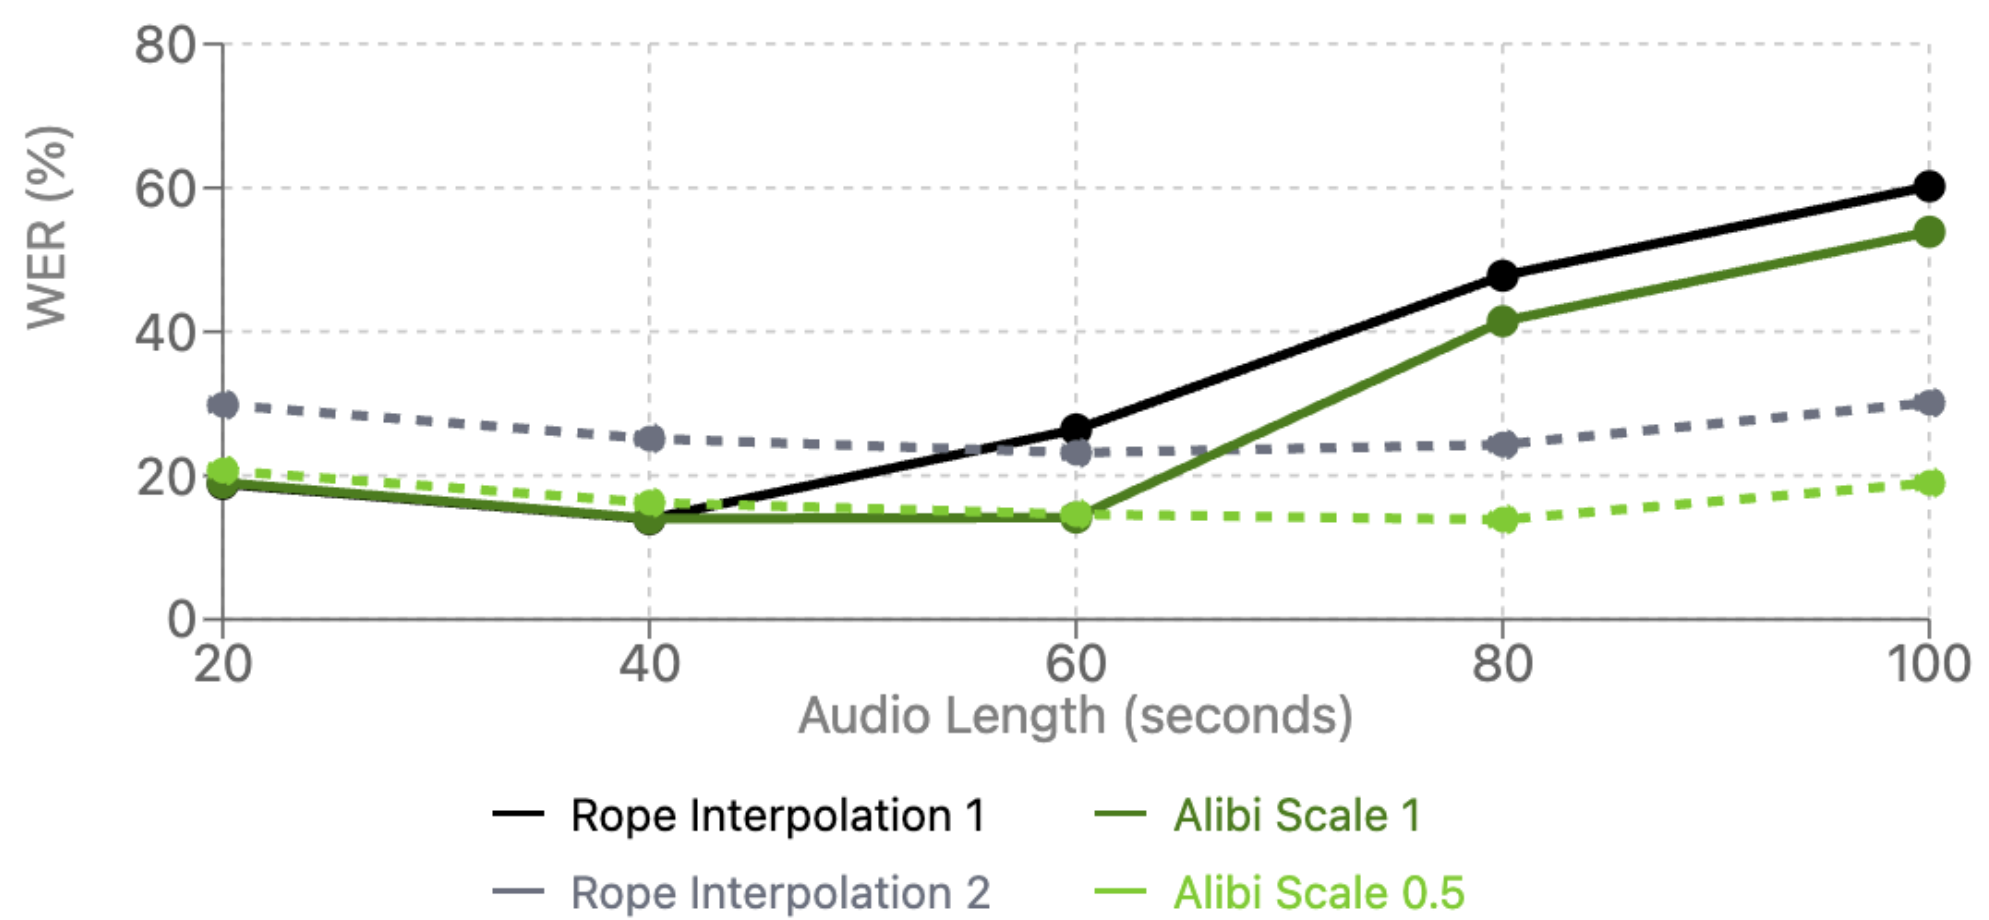
\includegraphics[width=0.8\textwidth]{images/alibi_vs_rope.png}
   \caption{Comparison of Attention with Linear Biases (ALiBi) and Rotary Position Embeddings (RoPE) on long-form ASR with the Earnings dataset. For RoPE, larger interpolation factors correspond to reducing the angular rotation step to better accommodate longer sequences. For ALiBi, smaller scaling factors apply a lighter penalty to distant tokens, allowing the model to attend further into the context.}
    \label{fig:alibi_rope}
\end{figure} 
To improve generalization for nGPT encoder architecture, we modified each positional encoding. For RoPE, we reduced the angular rotation applied at each position so that longer input sequences would span the same effective angular spectrum as those seen during training. For ALiBi, we adjusted the bias scaling factor, which controls how strongly distant tokens are down-weighted, thereby allowing the model to retain more attention to faraway context. These adjustments significantly reduced WER across all lengths. Nevertheless, ALiBi remained more effective than RoPE in long-context ASR, highlighting the benefit of incorporating distance-aware attention biases in encoder-style speech tasks.

Empirically, the two approaches demonstrated task-dependent behavior. In ASR, ALiBi showed improvements, likely because reducing emphasis on distant tokens is not detrimental for speech recognition, where local context dominates. In contrast, for AST, long-range context is more critical, and we found RoPE to be more effective. These results highlight that positional encoding strategies interact differently with downstream tasks: ALiBi favors efficiency in short-to-mid context alignment, whereas RoPE better supports tasks requiring global context retention.    
